\documentclass[french]{article}
\usepackage[utf8]{inputenc}
\usepackage[english]{babel}
\usepackage[T1]{fontenc}
\usepackage{babel}
\usepackage{amsmath}
\usepackage{graphicx}
\usepackage{hyperref}
\usepackage{mathtools}

\usepackage{biblatex}
\usepackage{algorithm}
\usepackage{algpseudocode}
\usepackage{siunitx}
\addbibresource{biblio.bib} 


\title{brouillon-pstl-bdd.v6}
\author{Alpha DIALLO, Lamine KEITA, Sacha MEMMI}
\date{Mai 2020}



\begin{document}


\maketitle
\begin{figure}[htp]
    \centering
    
\includegraphics[width=12cm, height=5cm]{logo_upmc}
    \label{fig:logo}
\end{figure}


\newpage
\tableofcontents
\newpage
\section{Abstract}


Les fonction booléennes sont très largement utilisées en science. Elles sont aussi largement utilisées parce que simple à manipuler et à mettre en place, leur utilité est également très large. 
\vspace{5mm} %5mm vertical space

Les structures avec lesquelles nous travaillons dans ce papier sont ce que l'on appelle des robdd, reduced ordered binary decision diagram. Elles représentent des fonctions booléennes en tant que diagramme avec leurs noeuds ordonnés et le nombre de ces noeuds réduit. Elles sont l'une des méthode préférée pour représenter les fonctions booléenne en particulier en informatique. Elles sont préférées car facile à implémenter, quelques ligne de codes dans n'importe quel langage sont suffisantes pour les représenter, mais également parce qu'elles sont simple à manipuler.
\vspace{5mm} %5mm vertical space

En particulier nous cherchons à énumérer le nombre de robdd unique représentant une fonction ayant un nombre définie de variable selon leurs tailles. Ce problème a intéressé le domaine scientifique depuis que ces structures ont vu le jour, il présente de nombreux intérêts dans tous les domaines où l'on travail avec des robdd.
\vspace{5mm} %5mm vertical space

Puis en plus de rappeler la méthode standard de génération des robdd, nous donnons un nouveau moyen d'obtenir ces structures. Nous obtenons par cette nouvelle méthode un générateur uniforme de robdd que nous pouvons appliquer à plusieurs types de tests.

\newpage


\section{Introduction}
L'idée derrière les diagrammes de décision binaires a été introduite par Shannon en 1938 dans \cite{shannon}. Les diagrammes de fonction binaires sont principalement des outils pour les ingénieurs (et autre professions travaillant dans le hardware en informatique) qui manipulent des circuit électroniques, cas où l'utilisation de tables de vérité se révèle efficace. Dans ce cas là diviser leurs circuits complexes en sous circuits simple comme le permettent les diagrammes de décision binaires (concept que l'on appelle "diviser pour régner") est très efficace. 

Plus particulièrement les circuits électroniques sont devenus si compliqués que les robdd sont à peine suffisant pour les traiter comme l'a noté Knuth il y a de ça plus de 10 ans \cite{knuth}.

Les fonctions booléennes ont de très nombreux usages, dans \cite{cahier} P. Camion convertie de nombreux problemes du domaine des entiers en problèmes équivalent en algèbre booléenne et dans ce même papier R. Fortet a introduit l'idée de colorer un graphe selon 4 couleurs (theoreme des quatres couleurs \cite{dirac}) en assignant deux variables booléenne à chaque vertex.

Un bdd (binary decision diagram) est un diagramme de décision binaire pouvant représenter une fonction booléenne, l'utilité des bdd ne se limite a représenter des fonctions booléenne mais dans ce papier nous nous limiterons à celle ci. Un robdd (reduced ordered binary decision diagram) est comme son nom l'indique la forme réduite et ordonné d'un bdd. Dans la literrature le terme bdd est presque toujours utilisé pour évoquer un robdd, nous différencierons tout d'abord entre ces deux termes pour mettre l'accent sur l'aspect réduction. Les bdd que nous considerons dans ce papier sont toujours ordonné, quand on parle de bdd nous faisons en fait référence à un obdd  (ordered binary decision diagrams).

Les robdd n'ont été introduit qu'en 1986 \cite{bryant_graph}. Assez tard dans l'histoire de l'informatique. Les robdd ont été une telle révolution que \cite{bryant_graph} est pendant des années resté le papier le plus cité dans la littérature scientifique, et de nombreuses autres variantes de robdd ont été crées depuis \cite{wegner}.

Le principe d'un robdd est simple, on cherche à conserver de l'espace mémoire en se débarrassant des structures redondantes, la mémoire étant une préoccupation importante en informatique. Pour réduire un bdd, nous supprimons les sous structures redondantes, nous supprimons également les noeuds non essentiels. Nous représentons les bdd en tant qu'arbre plat et les robdd en tant que dag (directed acyclic diagrams) \cite{flajolet_automata}. Plus généralement les robdd sont des sous types de bdd et tous les types de bdd peuvent être représentés par un dag.

\begin{figure}[htp]
    \centering
    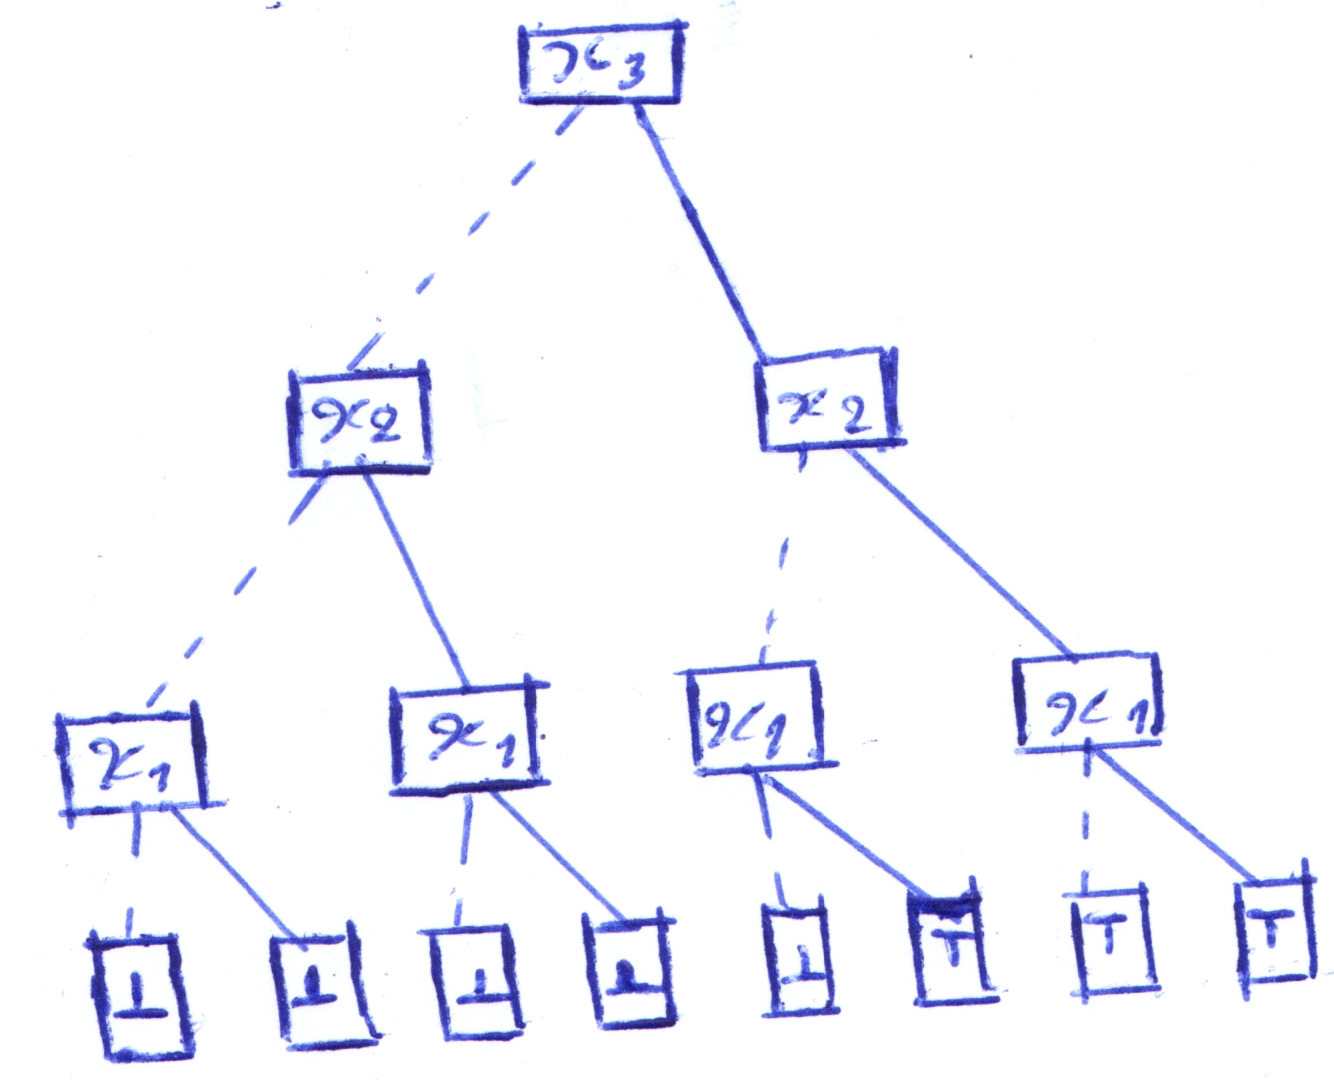
\includegraphics[width=6cm, height=6cm]{tree019}
    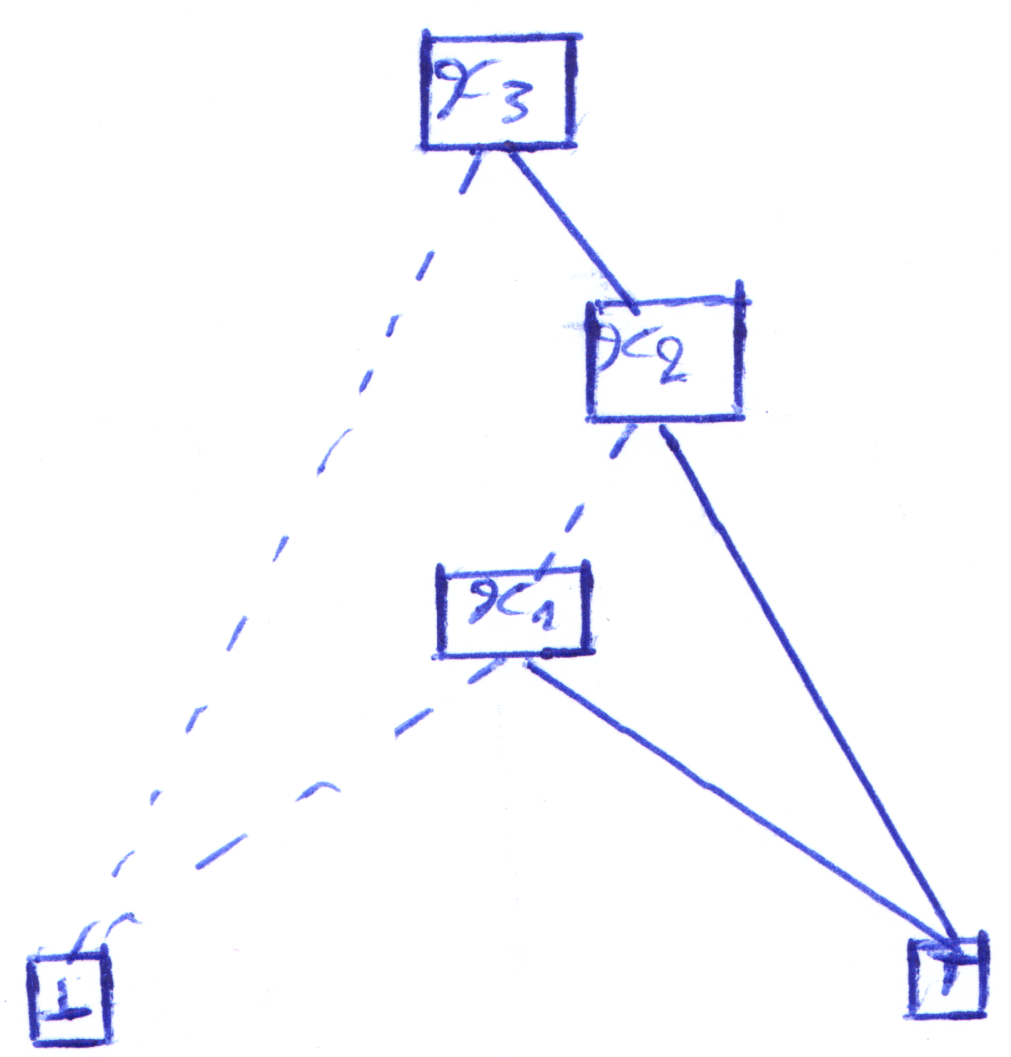
\includegraphics[width=6cm, height=6cm]{tree020}
    \caption{Arbre de decision binaire à gauche et dag représentant sa forme réduite}
    \label{fig:Figure1.1}
\end{figure}
\newpage
Un exemple d'arbre de décision binaire et un dag représentant sa forme réduite sont donné dans la figure 1. Nous suivons ici le consensus dans la littérature et représentons les liens vers les fils haut par une ligne solide, et ceux vers les fils bas par une ligne en pointillé.

En plus de l'utilité évidente des fonctions booléennes ont peut aussi noter que les bdd sont devenus aussi populaire parce que comme Knuth l'a noté dans \cite{knuth} les bdd simples sont relativement facile à fusionner pour obtenir des bdd plus complexes.

Dans ce rapport notre but est de présenter un nouveau procédé permettant d'énumérer des robdd sans passer par le processus de compression.

Le processus de compression est relativement simple avec une complexité P (polynomial), mais la méthode standard de génération des bdd d'un nombre donné de variable k utilisé jusqu'ici était impraticable pour {\(k > 4\)} \cite{newton}. Pour construire les bdd ayant k variable dans la méthode standard nous construisons tout d'abord toutes les fonctions booléennes ayant k variables, puis leurs bdd, puis compressons ces bdd afin d'obtenir leurs robdd et enfin nous supprimons les robdd apparaissant plus d'une fois. Ceci avait une complexité doublement exponentielle de  O(\( {2^2}^k\) ).

Nous définissons la taille d'un robdd par le nombre de noeuds internes (non terminaux) qu'il contient.
\newpage
Pour énumérer ces structures dans la méthode que nous introduisons ici nous utilisons de nombreuses propriétés des robdd.  Nous utilisons ensuite des méthodes dites de unranking et ranking basées sur le modèle standard introduit dans \cite{wilf} en définissant un ordre total sur les robdd et en décomposant chacun par une constitution de sous robdd.

Le processus de ranking consiste à attribuer à chaque objet d'un ensemble un identifiant unique, celui du unranking correspond au processus inverse, retrouver depuis son identifiant un objet au sein d'un ensemble.

Nous obtenons grâce à cette méthode un générateur uniforme de robdd.

Avec la méthode standard introduite dans \cite{newton} les robdd de taille proche de la taille maximal étaient crées avec une grande probabilité, mais dans celle ci chaque robdd a un identifiant unique dans l'ensemble. On peut également modifier ce générateur pour ne créer que des robdd ayant certaine classes de propriétés.

\begin{figure}[htp]
    \centering
    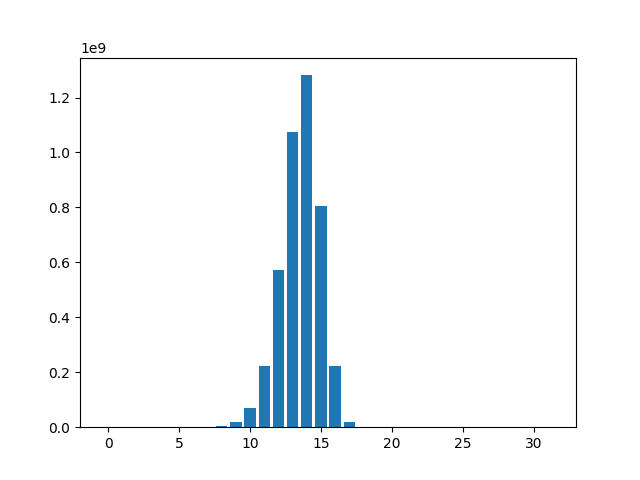
\includegraphics[width=11cm, height=8cm]{index5}
    \caption{Distribution des taille de bdd ayant 5 variable}
    \label{fig:Figure1.2}
\end{figure}

Avec notre méthode nous arrivons a comptabiliser les bdd ayant 5 variable, avec une implementation en python et un materiel limité, en 14 secondes.

Nos resultats sont similaire a ce qui etait estimé dans \cite{newton} pour 5 variable (on rapelle qu'ici on ne prend pas en compte les feuille dans le calcul de la taille d'un bdd).

Dans ce rapport nous considérerons que nous ne rencontrons jamais le robdd réduit au noeud unique \(\top\) ou \(\bot.\)
\newpage
\section{BDD et ROBDD}
Dans cette section nous cherchons à définir les structures basique avec lesquelles nous travaillons, les bdd et les robdd.

\begin{center}
\emph{“A Boolean function is a function in mathematics and logic whose arguments, as well as the function itself, assume values from a two-element set (usually \{0,1\}).”} 
\end{center}

- Wikipedia 
\vspace{5mm} %5mm vertical space

Il existe de nombreux moyens pour représenter des fonctions booléennes. Ceux préférés en science de l'informatique sont les diagrammes, pas seulement grâce à la manière dont ces diagrammes peuvent être réduit, mais aussi parce qu'ils peuvent être conservés en mémoire en tant que multiple noeuds qui ne sont pas forcement adjacent en mémoire les uns aux autres. Ceci rend leur conservation plus simple et efficace.

Un bdd est composé de noeuds ayant un label. Chaque noeud non terminal possède deux enfants, ou fils, un bas et un haut liés à leurs parents par des liens notés respectivement 0 et 1. Chaque noeud a un index qui détermine son ordre dans le bdd. Les noeuds sont traités dans l'ordre décroissants de leurs indexes.

La manière dont nous ordonnons les noeuds est importante comme noté dans \cite{newton} et trouver l'ordre le plus efficace est un problème NP (nondeterministic polynomial time). Nous savons que plus un bdd a de variable plus sa taille tend à se rapprocher de celles du robdd qui lui correspond.

La chose importante ici est que les bdd vu en pratique ont tendance à avoir au moins un ordonnancement efficace de leurs noeuds où la taille de leurs robdd est bien inférieur à la leurs \cite{gropl}. Raison pour laquelle déterminer l'ordre le plus efficace est aussi important.

La racine a un index k qui est l'index maximal de la bdd (ou robdd), et les noeuds terminaux ont des index nuls. Tous les noeuds internes (quand ils existent) ont des indexes allant de k à 0, non inclus. Pour un bdd l'index de la racine est le nombre de variables de la fonction booléenne qu'il représente, pas forcement pour un robdd.

Pour exécuter un bdd nous allons tout d'abord à la racine, puis nous suivons un chemin en se fiant à la valeur de chaque variable données en entrée selon l'index du noeud courant. Si la variable d'index du noeud courant est 0 nous nous rendons à l'enfant bas du noeud courant, l'enfant haut si la variable a pour valeur 1. Nous finissons par arriver à un noeud terminal, que dans le reste de ce papier nous appellerons feuille, de valeur \(\top\) (true) ou \(\bot\) (false) qui est la valeur de retour de la bdd pour les variables considérées.

Pour le bdd de la figure 1 si l'on donnait les variables 101 en tant qu'entrées elle retournerait \(\top\) (true). 
\newpage

La méthode classique pour obtenir un robdd est de réduire un arbre de décision binaire. Définissons maintenant comment on effectue cette réduction.

Pour effectuer cette réduction nous suivons tout d'abord deux règles, que nous notons R et M.

Considérons \(\Delta\) un dag représentant une fonction booléenne f. Considérons également \(\alpha\) et \(\beta\)  deux noeuds distincts dans \(\Delta\) .

\textbf{Règle M}: Si \(\alpha\) et \(\beta\) sont des racine de sous graphes isomorphes alors fusionner \(\beta\) et \(\alpha\).

\textbf{Règle R}: Si les deux fils de \(\beta\) sont isomorphes à \(\alpha\), alors faire pointer tous les liens entrant de \(\beta\) vers \(\alpha\) et supprimer \(\beta\).

Nous appliquons récursivement ses deux règles à tous les noeuds de \(\Delta\) .
\vspace{5mm} %5mm vertical space

Deux ordres de parcours peuvent être considérés, \(post_{o}\) et \(pre_{o}\).

Dans le \(post_{o}\) nous visitons tous d'abord le fils bas du noeud courant, puis son fils haut et enfin le noeud lui-même.
Dans le \(pre_{o}\) nous visitons tous d'abord le neoud courant, puis son fils bas, et enfin son fils haut.

Nous choisissons ici de considérer l'ordre de traversé \(post_{o}\) pour effectuer chacune de nos compressions, puisque c'est celui préféré en science de l'informatique. Choisir un ordre en particulier est important pour s'assurer que des bdd équivalents soient compressés en tant que robdd identique une fois l'ordre des variables établie.
\vspace{5mm} %5mm vertical space

Nous pouvons désormais définir formellement le processus de compression.

\textbf{Compression} :  Considérons \(\Delta\) le bdd de la fonction f.  Quand le noeud \(\lambda\) est visité, \(\lambda\) étant l'enfant d'un noeud \(\mu\). Si un sous-arbre \(\Lambda\), celui qui a pour racine \(\lambda\), a déjà été vu lors de la traversé de \(\Delta\), sous arbre dont la racine est \(\omega\), alors \(\Lambda\) est supprimé de \(\Delta\) et le noeud \(\mu\) obtient un pointeur vers \(\omega\), remplaçant le lien allant précédemment de \(\mu\) à \(\lambda\). Une fois que la traversé de \(\Delta\) achevé, le dag résultant est le robdd de f.

Voir Appendix \ref{Appendix_1} pour l'algorithme de compression.
\vspace{5mm} %5mm vertical space

Définissons maintenant formellement un robdd.

Considérons un robdd \(\Delta\) = (Q, I, r, \(\delta\)). Q est l'ensemble de noeuds que l'on obtient par une traversé en \(post_{o}\) de \(\Delta\). r est la racine de \(\Delta\), I est la fonction qui associe pour tout noeud \(\lambda\) \(\in\) Q son index et \(\delta\) est la fonction de transition complète qui associe à chaque noeuds ses fils.
\begin{itemize}
    \item
    	Q  =   ([feuille1],[feuille2], …, r)
    	([feuille1] etant la premiere feuille que l'on rencontre lorsque l'on parcourt \(\Delta\) en \(post_{o}\) et [feuille2] la seconde)
    \item 
        \(I = Q   \rightarrow  \{0, \ldots , k\}\) où k est l'index de r
    \item 
       \( \delta = (Q \setminus  \{\top,  \bot\}) * \{0, 1\} \rightarrow \) Q
\end{itemize}

On note que Q a une taille forcement superieur ou egal à 3.

On peut ainsi representer le dag de la figure 1 par un robdd \(\Delta\) = (Q, I, r, \(\delta\)) ayant les propriétés suivantes:
\begin{itemize}
    \item
    	Q  =   \((\bot, \top, x1,x2,x3)\)
    \item 
        \(I = \{\bot, \top, x1,x2,x3\}   \rightarrow  \{0,0,1,2,3\}\)
    \item 
       \( \delta = \{ x1 * 0 \rightarrow \bot , x1 * 1 \rightarrow \top, x2 * 0 \rightarrow x1, x2 * 1 \rightarrow \top, x3 * 0 \rightarrow \bot, x3 * 1 \rightarrow x2 \} \) Q
    \item 
        r = x3
\end{itemize}

Dans le reste de ce papier nous utiliserons le terme bdd pour faire référence aux robdd.

\section{(RO)BDD : propriétés}
Dans cette section nous définissons des propriété que l'on assigne aux bdd. Pour ce faire nous mettant en place un ensemble de notation et d'opérations. Toute les notations utilisés dans cette section seront utilisés dans le reste de ce rapport. Les opérations que nous définissons pour les listes sont également applicables aux ensembles.
\vspace{5mm} %5mm vertical space

Pour deux noeuds \(\alpha\) et \(\beta\) d'un dag \(\Phi\) nous écrivons \(\alpha\) \(\Leftarrow_{post}\) \(\beta\) si le neoud \(\alpha\) est visité avant le noeud \(\beta\) en \(post_{o}\) lors de la traversé de \(\Phi\), et \(\alpha\)\(\Leftarrow_{pre}\) \(\beta\) si le noeud \(\alpha\) est visité avant le noeud \(\beta\) en \(pre_{o}\) lors de la traversé de \(\Phi\).
\vspace{5mm} %5mm vertical space

Pour deux listes l et l’ de tailles respectives m et n, où l = (p0,p1…,pm) et l’ = (p’0,p’1,…,p’n) nous écrivons L=l+l’ l'opération telle que si m\(<\)n avec L=(P0,P1,…,Pn) alors nous avons pour \(i\leq\) m Pi=pi+p’i et pour \(m<i\leq n\) Pi=p’i.

Pour une liste l nous notons \(\mid l\mid \) le nombre d'élément dans l, et \(\mid\mid l\mid\mid\) la somme de tous ses éléments.
\vspace{5mm} %5mm vertical space

\textbf{Profil d'un ensemble}: Le profil P=profil(S) d'un ensemble S est simplement une liste du nombre d'élément de S ayant un certain index, on note P = (p0,p1…,pj,…pk) où pj est le nombre d'elements dans l'ensemble S d'index j et k l'index maximal de S. 

Le processus d'extension de cette définition de profil à des graphes est évident.
\vspace{5mm} %5mm vertical space

\textbf{Spine d'un bdd} : Considérons un bdd \(\Delta\) = (Q, I, r, \(\delta\)) enraciné en r. Le spine T = (Q’, I, r, \(\delta\)’) de \(\Delta\) est un dag tel que Q’ = Q / \{\(\top,\bot\)\} où chaque noeud \(\lambda\) \(\in\) Q’ a été obtenu par la traversée en \(post_{o}\) de \(\Delta\) en faisant omission des deux feuilles. Les liens du spine sont décrit en utilisant une fonction de transition partielle \(\delta\)’: Q’ \(\times\) \{0, 1\} \(\rightarrow\) Q' \(\cup\) \{nil\} où nil est un symbole spécial désignant une transition non définie.

Décrit simplement un spine est un bdd auquel on retire les deux feuilles et les pointeurs.

Dans le reste de ce papier nous nous référerons aux valeurs non définis de la fonction de transition partielle en tant que nil transition.
\vspace{5mm} %5mm vertical space

Nous notons n le nombre de noeud d'un dag \(\Delta\) d'un bdd, nous savons que son spine S a le même nombre de noeud que \(\Delta\) à l'exception des deux feuilles. Nous pouvons ainsi noter que S a (n-2) noeuds. Nous savons également que tous les noeuds non terminaux de \(\Delta\) ont deux enfants, ainsi le nombre de transition dans \(\Delta\) est (n-2)*2, ce qui est le nombre total de transition dans S (a la fois les transition nil et non nil). Nous savons également que chaque noeud \(\lambda\) \(\in\) S a nécessairement un degré entrant de 1 à l'exception de la racine ainsi le nombre restant de transition non nil dans S est (n-3). Nous pouvons maintenant conclure que S a un nombre de nil transition égal à (n-1).
\vspace{5mm} %5mm vertical space

\textbf{Sous arbre} : Un sous arbre TA(\(\lambda\)) est un arbre enraciné en \(\lambda\) appartenant à un autre arbre.

\textbf{Pool} : Considérons un dag D, la pool PT(\(\lambda\)) d'un noeud \(\lambda\) \(\in\) D est:

\begin{center}
PT(\(\lambda\)) = \{\(\tau\)’ \(\in\) D \(\mid\)  \(\tau\)’ \(\Leftarrow_{pre}\) \(\lambda\) et I(\(\tau\)’) \(<\) I(\(\lambda\))\} \(\cup\) \{\(\top\), \(\bot\)\} .
\end{center}

\textbf{Pool profil} : Le pool profil de \(\lambda\) est comme son nom l'indique le profil de sa pool que l'on note: profil(PT(\(\lambda\))). 

\textbf{Level set} : Considérons un dag D, le level set \(\lambda\) \(\in\) D est:
\begin{center}
ST(\(\lambda\)) = \{\(\theta\)’ \(\in\) D \(\mid\) \(\theta\)’ \(\Leftarrow_{pre}\) \(\lambda\) et I(\(\theta\)’) = I(\(\lambda\))\} . 
\end{center}
\textbf{Level rank} : Considérons ST(\(\lambda\)) le level set du noeud \(\lambda\), nous écrivons RS(\(\lambda\)) son sibling rank tel que:
\[ RS(\lambda) = \mid ST(\lambda)\mid \]
\newpage
\begin{figure}[htp]
    \centering
    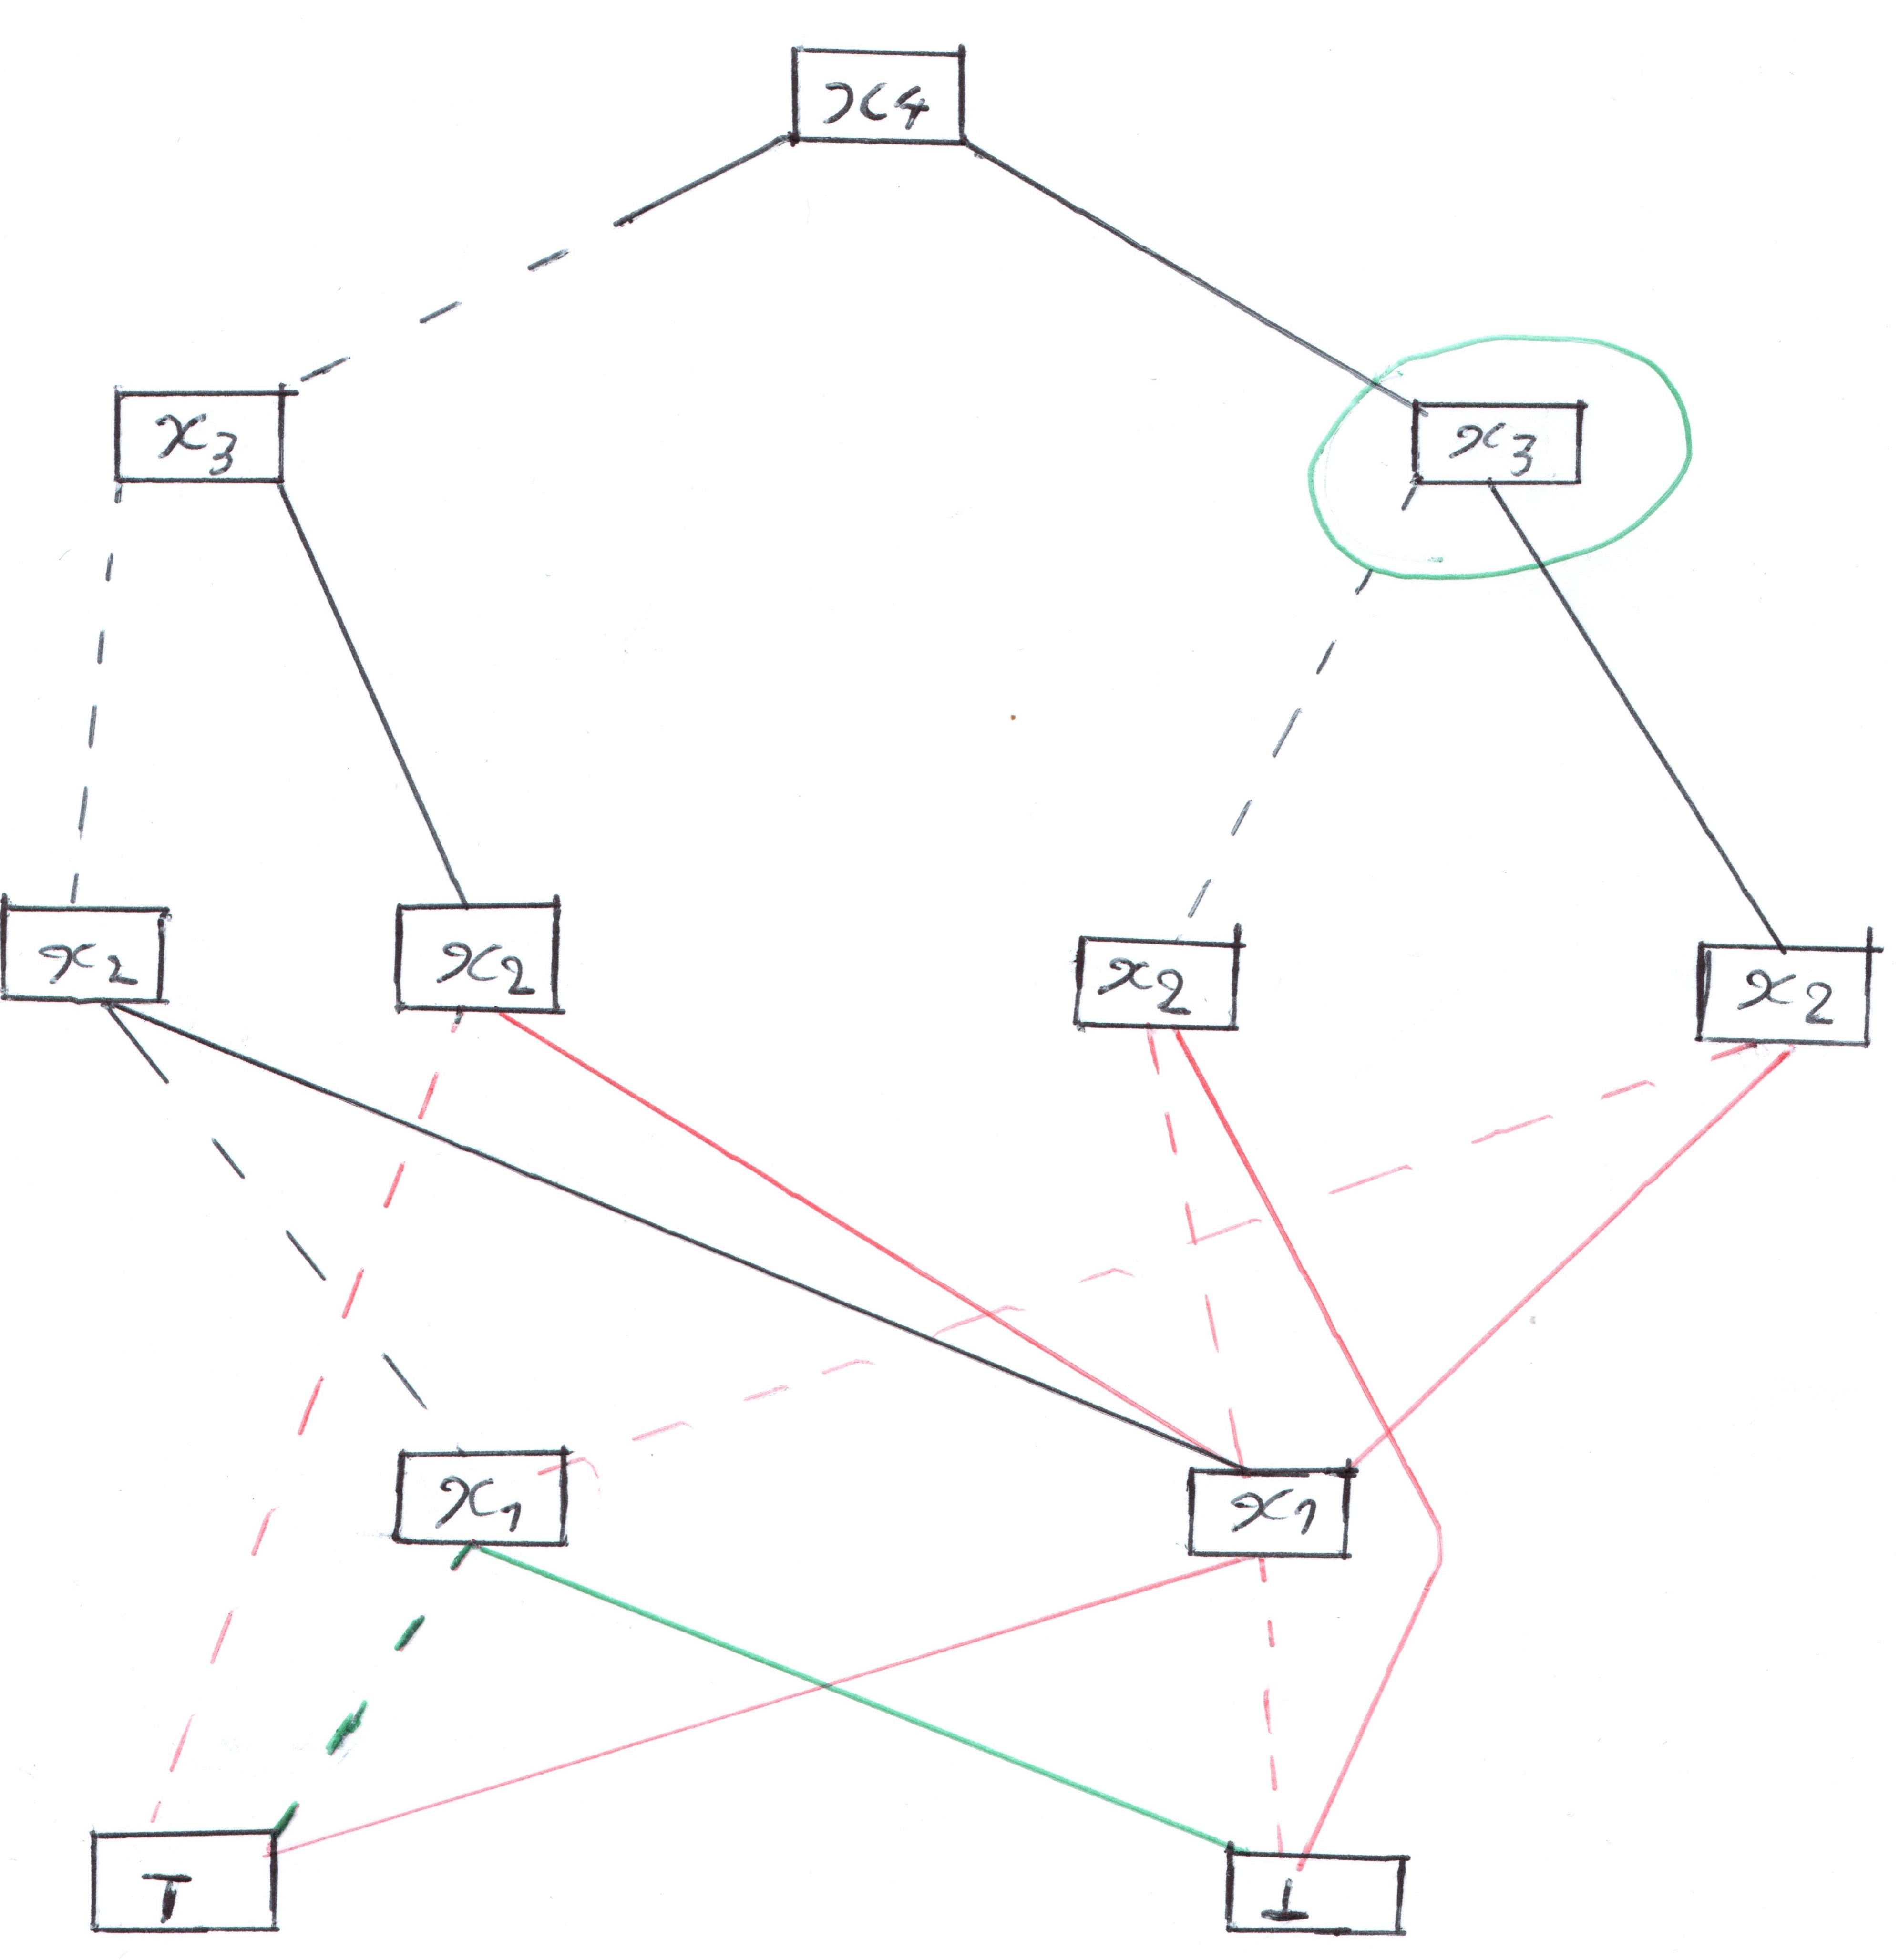
\includegraphics[width=11cm, height=12cm]{tree21}
    \caption{Dag}
    \label{fig:Figure2}
\end{figure}
On considère dans la figure 3 un dag. Les pointeurs sont représentés en rouge. Le spine du robdd de ce dag est le graphe réduit aux transitions en noirs.

La pool du noeud entouré en vert est : \(\{x_2,x_2,x_1,x_1,\top,\bot\}\). 

Le profil de ce dag est : \{2,2,4,2,1\}.

\vspace{5mm} %5mm vertical space

Nous savons de la manière dont nous définissons les bdd que pour être valide un bdd \(\Beta\) doit avoir les propriétés suivantes:

FACT 1.1 : \emph{De la règle r nous faisons la conclusion que deux noeuds de même index ne peuvent avoir les même descendants, autrement ils auraient été fusionnés.}

FACT 1.2 : \emph{A partir de la règle m nous savons qu'un noeud ne peut avoir deux enfants identiques, autrement ce noeud aurait été supprimé.}

\newpage
\section{Comptage}
La méthode classique permettant d'énumérer les bdd ayant un nombre de variable k et une taille n est la suivante:
\begin{enumerate}
    \item 
	Énumérer toute les \({2^2}^k\) fonctions booléennes et dresser leurs arbres de décision binaires
	\item
	Appliquer le processus de compressions pour obtenir leurs bdd
	\item
    Filtrer les bdd de taille n
	\item
	Supprimer les bdd réapparaissant plus d'une fois afin de ne conserver qu'une seule de leurs occurrence
\end{enumerate}
Nous proposons ici une méthode récursive permettant d'effectuer cette énumération sans passer ni par le processus de compression ni celui de filtration. Ces deux processus sont hautement coûteux avec une complexité doublement exponentielle \(O(2^{2^{k}})\).
\vspace{5mm} %5mm vertical space

\textbf{Proposition 1} :  Considérons T = (Q’, I, r, \(\delta\)’) un spine avec un ensemble de noeuds Q’, racine r et fonction de transition partiel \(\delta\)’ : Q’ \(\times\) \{0, 1\} \(\rightarrow\) Q’ \(\cup\) \{nil\}. La fonction de transition entière \(\delta\) : Q’ \(\times\) \{0, 1\} \(\rightarrow\) Q’ \(\cup\) \{\(\top\), \(\bot\)\} est la fonction de transition d'un bdd avec un spine T si et seulement si pour tout noeuds \(\lambda\) \(\in\) Q’, noté \(\lambda\)0 = \(\delta\)(\(\lambda\), 0) et \(\lambda\)1 = \(\delta\)(\(\lambda\), 1), la paire (\(\lambda\)0, \(\lambda\)1) satisfait : 
\begin{enumerate}
    \item 
	Si \(\delta\)’(\(\lambda\), 0) != nil et \(\delta\)’(\(\lambda\), 1) != nil alors 
	\begin{center}
	\(\lambda\)\(\sigma\) = \(\delta\)’(\(\lambda\), \(\sigma\)) pour \(\sigma\) \(\in\) \{0, 1\}.
    \end{center}
    \item
	Si \(\delta\)’(\(\lambda\), 0) = \(\delta\)’(\(\lambda\), 1) = nil, alors 
	\begin{center}
	\(\lambda\)\(\sigma\) \(\in\) PT(\(\lambda\))  pour \(\sigma\) \(\in\) \{0, 1\} et \(\lambda\)0 != \(\lambda\)1, et il n'y a aucun noeud \(\lambda\)’ != \(\lambda\) avec I(\(\lambda\))=I(\(\lambda\)’) tel que \(\delta\)(\(\lambda\)’, ·) = \(\delta\)(\(\lambda\), ·).
    \end{center}
    \item
	Si \(\delta\)’(\(\lambda\), 0) = nil et \(\delta\)’(\(\lambda\), 1) != nil, alors
	\begin{center}
	\(\lambda\)0 \(\in\) PT(\(\lambda\)) et \(\lambda\)1 = \(\delta\)’(\(\lambda\), 1).
	\end{center}
    \item
	Si \(\delta\)’(\(\lambda\), 0) != nil et \(\delta\)’(\(\lambda\), 1) = nil, alors 
	\begin{center}
	\(\lambda\)0 = \(\delta\)’(\(\lambda\), 0) et \(\lambda\)1 \(\in\) PT(\(\lambda\)) \(\cup\) TA(\(\lambda\)0) \(\setminus\) \(\lambda\)0 .
    \end{center}
\end{enumerate}
\newpage
Preuve. Puisque \(\delta\)(·, ·) doit étendre \(\delta\)’(·, ·), le cas 1. est triviale puisque nous devons étendre la fonction de transition uniquement où l'on a \(\delta\)(\(\lambda\), \(\sigma\)) = nil. Dans le cas 2., nous devons choisir pour (\(\lambda\)0, \(\lambda\)1) deux noeuds dans PT(\(\lambda\)). De plus \(\lambda\)0 != \(\lambda\)1 comme déclaré dans FACT 1.2 et un autre noeud avec le même index que \(\lambda\) ne peut pas avoir les même enfants (\(\lambda\)0, \(\lambda\)1) comme déclaré dans FACT 1.1. Dans le cas 3., l'enfant bas doit être choisie dans la pool de \(\lambda\) puisque l'on doit préserver le spine. Dans le cas 4., l'enfant haut de \(\lambda\) est aussi choisi dans la pool de  \(\lambda\) ou dans TA(\(\lambda\)0) (et doit être diffèrent de \(\lambda\)0).
\vspace{5mm} %5mm vertical space

Nous définissons maintenant un procédé permettant de calculer le nombre de bdd correspondant à un spine donné, nous appellerons le nombre de bdd correspondant à un spine S le poids de S.

\textbf{Poids d'un noeud} : Considérons un spine T = (Q’, I, \(\delta\)’, r), le poids wT(\(\lambda\)) d'un noeud \(\lambda\) \(\in\) Q’ est le nombre de transition possible pour compléter la fonction de transition partielle \(\delta\)’(\(\lambda\), ·) et former un bdd valide de spine T.

\textbf{Proposition 2} (Poids d'un noeud) : Considérons T = (Q’, I, \(\delta\)’, r) un spine , le poids wt(\(\lambda\)) d'un noeud \(\lambda\) \(\in\) T est:

\begin{equation}
    wt(\lambda) =
    \begin{cases}
        1 & \text{si \(\delta\)’(\(\lambda\), 0) != nil et \(\delta\)’(\(\lambda\), 1) != nil}\\
        pts(\lambda) (pts(\lambda) - 1) - ST(\lambda) & \text{si \(\delta\)’(\(\lambda\), 0) = \(\delta\)’(\(\lambda\), 1) = nil}\\
        pts(\lambda) + pts0(\lambda) - 1  & \text{si \(\delta\)’(\(\lambda\), 0) = nil et \(\delta\)’(\(\lambda\), 1) != nil}\\
        pts(\lambda)   & \text{si \(\delta\)’(\(\lambda\), 0) != nil et \(\delta\)’(\(\lambda\), 1) = nil}
    \end{cases}       
\end{equation}

Avec pts(\(\lambda\)) = \(\mid\mid profil(PT(\lambda)) \mid\mid\) et pts0 = \(\mid\mid profil(TA(\delta \textquoteright(\lambda,0))) \mid\mid\).

Preuve. A partir de la proposition 1 nous énumérons tous les liens possibles (liant à un noeud) nous pouvons utiliser pour compléter la fonction de transition partielle. Dans le premier cas nous ne pouvons compléter que avec les liens déjà existant (comme déclaré dans 1) de proposition 1) le cas est déjà définie). Dans le second cas nous énumérons tous les liens possible de 2) de la proposition 1. Dans le troisième et quatrième cas nous faisons la même chose pour respectivement  3) et 4).
\vspace{5mm} %5mm vertical space

Le poids d'un sous arbre est le poids cumulé de ses noeuds.

\textbf{Poids d'un spine} : Considérons un spine T = (Q’, I, \(\delta\)’, r), le poids W(T) de T est le poids cumulé de ses noeuds.
\[W(T) = \prod wt(\lambda) \mid \lambda \in Q\textquoteright\]


Dans le cas où le poids d'un noeud \(\lambda \in Q\textquoteright\) est nul ou négative nous savons que le spine T est invalide parce que T n'est pas le spine du moindre bdd. Ceci arrive uniquement lorsque \(\lambda\) a ses deux enfants égaux à nil (puisque l'on a nécessairement \(\mid\mid profil(PT(\lambda)) \mid\mid \geq\)2).

Cette formule peut être aisément décrite de manière récursive, via une traversée en \(post_{o}\) où toutes les informations nécessaires pour calculer le poids du noeud ont déjà été traités.
\vspace{5mm} %5mm vertical space

Nous notons \(T_{nk}\) l'ensemble des spine de taille n et de nombre de variable k, et \(N_{nk}\) le nombre de bdd de taille n et de nombre de variable k.
Pour déterminer \(N_{nk}\) tout ce que nous avons à faire est déterminer la totalité des spine de taille n et de nombre de nombre de variable k et ensuite déterminer leurs poids, nous faisons ensuite l'addition de leurs poids.

\[N_{nk} = \sum W(T) \mid T \in T_{nk}\]

\section{Combinatoire sur les spine}
Ce que nous voulions dans la section précédente était d'énumérer tout les bdd de taille n et de nombre de variable k. Pour ce faire nous devons déterminer les spine de taille n et de nombre de variable k. Ceci n'est un processus aisé à informatiser.

Nous définissons ici un processus récursive où nous construisons les spine par chacun de leurs noeuds et des que l'on a déterminé que ses spine ne sont pas valides on les ignore. 
\vspace{5mm} %5mm vertical space

Nous définissons un spine Tt en tant que tuple tel que:
\[Tt = T\textquoteright \cup N_i \cup T\textquoteright\textquoteright \mid nil \]
où \(N_i\) est un noeud d'index i, ceci signifie que le spine est soit reduit à nil soit à une racine et deux spine. Nous designerons dans la suite les spine T' et T'' qui composent Tt par le terme de sous spine.

Pour considerer un spine enraciné en r en particulier nous prendrons en compte trois de ses paramètres. Sa pool pT(T), le level rank de sa racine ST(r) et sa taille que nous designerons par \(\mid\mid T\mid\mid\).

Ces paramètre sont important parce qu'ils sont ce dont on a besoin pour déterminer le poids des spine que nous considérons.

Nous utiliserons la notation \(T_{m,p,s} \) pour considérer le spine enraciné en r de taille m (m =  \(\mid\mid T\mid\mid\)), de pool profil p (p = profil(pT(r))) et de level rank s (s = ST(r)) représenté par un tuple Tt tel décrit plus haut.


\textbf{Proposition 3} :  Pour \(T_{m,p,s} \) nous considérons des tailles pour chaque sous spine T’ \(\cup\) T’’ \(\in\) T de respectivement i et m – 1 – i, avec \(0\leq i\leq m-1\). Pour chacune des tailles de sous spine considérés nous considérons chacune des valeurs d'index que l'on peut assigner à leurs racines.

Nous avons ainsi un algorithme où nous considérons toute les tailles possible ainsi que les indexes des sous-spines, le level rank de la racine étant déjà donné par le pool profil du spine courant (ainsi que par le profil de T' dans le cas du level rank de T''). k correspond dans la suite à la taille de p.
\newpage
\begin{enumerate}
    \item Si m>0
        \begin{enumerate}
            \item
            \(T\textquoteright \in \underset{k_0\in K}{\bigcup} T_{i,p[:k_0-1],p_{k_0-1}} \)
            \item
            \(T\textquoteright\textquoteright \in \underset{k_0\in K}{\bigcup} T_{j,p1[:k_0-1],p1_{k_0-1}} \)
            \item
            \(W(T)=WTP(N_k,T\textquoteright,T\textquoteright\textquoteright)*W(T\textquoteright)*W(T\textquoteright\textquoteright)\)
        \end{enumerate}
 
    \item Si m = 0
        \begin{enumerate} 
            \item
            T=nil 
            \item
            W(T)=1
        \end{enumerate}
\end{enumerate}
Avec j = m-1-i, on note p[:i]=(\(p_0,p_1...p_i\)) pour designer dans un ensemble p que l'on ne considere que les elements ayant un index plus petit ou egale à i et \(p_{k}\) lorsqu'on designe l'element d'index k. On a egalement p1=p+profil(TA(T')) et K = \{0,1,...,k\}. Enfin on note W(T) le poids du spine T et WTP(N,T',T'') le poids du noeud N qui a pour fils bas le spine T' et pour fils haut le spine T''.
\vspace{5mm} %5mm vertical space

Avec algorithme nous ne considérons pour chaque récursion que les spine de même valeurs m, p et s. 
En s'inspirant de ce procédé on peut écrire un algorithme COUNT(m,p,s) prenant en argument une taille de spine m, un profil p et un level rank s et retournant un dictionnaire où chaque clé est le profil d'un spine et la valeur la somme des poids des spine ayant ce profil. 

Quelques exemples d'execution de la fonction COUNT:
\begin{itemize}
    \item COUNT(3,(2,0,0),0) nous retourne \{(0,1,1,1): 56, (0,2,0,1): 2, (0,0,2,1): 2\}
    \item COUNT(2,(2,0),0) nous retourne  \{(0,1,1): 8\}
    \item COUNT(1,(2),1) nous retourne \{(0,1): 1\}
    \item COUNT(1,(2),0) nous retourne \{(0,1): 2\}
\end{itemize}

Dans le premier cas le dictionnaire retourné nous indique qu'il existe 56 spine unique de taille 3 ayant pour profil (0,1,1,1), 2 ayant pour profil (0,2,0,1) et encore 2 ayant pour profil (0,0,2,1).

\vspace{5mm} %5mm vertical space

S'appuyant sur l'algorithme COUNT on definit N(n,k) qui renvoie le nombre de bdd de taille n et d'index k:
\[N(n,k)=\underset{(t,w)\in COUNT(n-2,(2,0,...,0),0)}{\sum} w\]

\(e^{(k)}\) est une liste de k+1 composants tous nul sauf le dernier qui est egal à 1 tel que \(e^{(k)} = (0,0,...,1)\).

La complexité de l'algorithme COUNT est exponentionel de l'ordre de \(O(2^{3k^2/2+k})\).

On decrit l'algorithme COUNT en pseudo code ci-dessous.
\begin{algorithm}
  \begin{algorithmic}[1]
    \Statex
    \Function{COUNT}{m,p,s}
      \State \Let{$d\gets \{\}$}
      \State \Let{$k\gets $Len(p)-1} \Comment{Len(p): renvoie la taille de la liste p}
      \If{m=0}
        \State \Let{$S\gets (\sum_{k-1}^{j=0} p_j)(\sum_{k-1}^{j=0} p_j-1)$}
        \If{$S>0$}
            \State \Let{$d \gets \{e^{(k)}:S\}$}
        \EndIf
      \Else
        \For{$i \gets$ 0 to m$-1$}
            \State \Let{$d_0\gets \{\}$}
            \If{i=0}
                \State \Let{$d_0 \gets \{():\sum_{k-1}^{i=0} p_i\}$}
            \Else
                \For{$k_0 \gets$ 1 to $k-1$}
                    \State \Let{$d_0 \gets d_0 \cup $COUNT$(i,p[:k_0-1],p_{k_0})$}
                \EndFor
            \EndIf
            \For{$(l,w_0) \gets d_0$}
                \State \Let{$d_1\gets \{\}$}
                \State \Let{$p\textquoteright \gets p+l$}
                \If{n-1-i=0}
                    \State \Let{$d_1 \gets \{():-1+\sum_{k-1}^{i=0} p_i\textquoteright\}$}
                \Else
                    \For{$k_1 \gets 1$ to $k-1$}
                        \State \Let{$d_1 \gets d_1 \cup $COUNT$(n-1-i,p'[:k_1-1],p'_{k_1})$}
                    \EndFor
                \EndIf
                \For{$(r,w_1) \gets d_1$}
                    \State \Let{$w \gets w_1*w_0$}
                    \State \Let{$t \gets l+r+e^{k}$}
                    \If{$t\in d$}
                        \State \Let{$d[t] \gets d[t]+w$}
                    \Else
                        \State \Let{$d \gets d \cup \{t:w\}$}
                    \EndIf\EndFor\EndFor\EndFor\EndIf
      \State \Return{$d$}
    \EndFunction
  \end{algorithmic}
\end{algorithm}
\newpage
\section{Unranking}
Notre approche pour le unranking s'appuie sur la méthode introduite dans \cite{wilf} où l'on decompose un arbre binaire en ses sous arbre gauche et droits et en attribuant à chaque décomposition un ordre total pour un bdd de taille et d'index fixé.

En s'inspirant de la Proposition 3 on definie une methode recursif b permettant de determiner le nombre d'arbres binaire ayant une certaine taille n.

\begin{equation}
    b_n =
    \begin{cases}
        1 & \text{si n = 0}\\
        \sum_{k=0}^{n-1}b_k*b_{n-1-k}  & \text{sinon}\\
    \end{cases}      
\end{equation}

En s'appuyant sur cette methode on peut definir une decomposition sur un arbre de taille fixé n. Cette methode s'apuie sur le fait que \(b_n\) est definie en une somme de produit, où chaque element du produit peut être vu comme la representation d'un arbre ayant un sous arbre gauche et un sous arbre droit de taille fixe. Par exemple \(B_7\) = 429, et on peut le decomposer en:
\[B_7=B_0*B_6+B_1*B_5+B_2*B_4+B_3*B_3+B_4*B_2+B_5*B_1+B_6*B_0\]
\[429=1*132+1*42+2*14+5*5+14*2+42*1+132*1\]

Où \(B_2*B_4\) represente un arbre composé d'un sous arbre droit de taille 4 et d'un sous arbre gauche de taille 2.

Ainsi, si je cherche l'arbre n\si{\degree}250, j'obtiens : 250 = 132 + 42 + 28 + 25 + 23. On trouve donc que l'arbre 250 est composé
d'un enfant gauche de taille 4 et d'un enfant droit de taille 2. Et plus particulièrement, parmi les 28 arbres ayant cette
décomposition 4x2, c'est l'arbre numéro 23 qui nous intéresse.


Pour ensuite retrouver le numero des sous arbre gauche et droit on procede comme ceci:
\begin{itemize}
    \item 23 //\( B_2 \) pour le numero du sous arbre gauche
    \item 23 \% \(B_2\)   pour le numero du sous arbre droit
\end{itemize}

En s'inspirant de cette methode on definie une fonction DECOMPOSE(r\textquoteright,n\textquoteright,s,p\textquoteright) permettant de generer un bdd de taille n\textquoteright, ayant un profil p\textquoteright et un rang r\textquoteright. s est une variable contenant le spine du bdd a generer.

\begin{algorithm}
  \begin{algorithmic}[1]
    \Statex
        \Function{decompose}{$rank, n, spine, p$}
            \State \Let{$p\_target \gets $list$(p)$} 
            \State \Let{$r \gets rank$}
            \State \Let{$s \gets spine.$get\_profil$()$}
            \State \Let{$k \gets $len$(p\_target)-1$}
            \State \Let{$q \gets s[:k]$}
            \State \Let{$q[0] \gets 2$}
            \State \Let{$i \gets  n-1$}
            \While{$i \geq 0$}
                \If{$i = 0$}
                    \State \Let{$d0 \gets {(): $sum$(q,1,k-1)+2}$}
                \Else
                    \State \Let{$d0 \gets \{\}$}
                    \For{$k0 \gets $range$(1,k)$}
                        \State \Let{$d0.$update$($count$(i,q[:k0],q[k0]))$}
                    \EndFor
                \EndIf
                \For{$(l,w0)$ in $d0.$items$()$}
                    \State \Let{$q\_prim \gets $sum\_profil$(q,l) $}
                    \If{$n-1-i = 0$}
                        \State \Let{$d1 \gets \{():$sum$(q\_prim,1,k-1)+1\}$}
                    \Else
                        \State \Let{$d1 \gets \{\}$}
                        \For{$k1$ in range$(1,k)$}
                        \State \Let{$d1.$update$($count$(n$-$1$-$i,q\_prim[:k1],q\_prim[k1]))$}
                        \EndFor
                    \EndIf
                    \For{$(h,w1)$ in$ d1.$items$()$}
                        \State \Let{$t \gets $sum\_profil$($sum\_profil$($e\_k$(k),$list$(l)),$list$(h))$}
                        \State \Let{$w \gets w0*w1$}
                        \If{$t = p\_target$}
                            \If{$w > 0$}
                                \State \Let{$r \gets r - w$}
                            \EndIf
                            \If{$r < 0$}
                                \State \Let{$r  \gets r + w$}
                                \State \Let{$r0 \gets r \% w0$}
                                \State \Let{$r1 \gets r // w0$}
                                \State \Return{$(i,r0,l,r1,h)$}
                            \EndIf
                        \EndIf
                    \EndFor
                \ENDFOR
                \State \Let{$i \gets i - 1$}
  \end{algorithmic}
\end{algorithm}
\newpage

On decrit ensuite une fonction GENERATE(r,n,s,p) permettant de generer un spine de taille n, de profil p et de rang r. La variable s est une variable globale qui contiendra en fin d'execution le bdd generé.
Cette fonction prend en argument un spine s contenant les noeuds initialement dans la pool (ici \(\up\) et \(\bot\)) et crée au fur et a mesure le bdd souhaité en faisant appel à la fonction decompose et en mettant à jour le spine.

\begin{algorithm}
  \begin{algorithmic}[1]
    \Statex
        \Function{generate}{$rank, n, spine, p\_target$}
            \State \Let{$k \gets $len$(p\_target)-1$}
            \If{$n = 0$}
                \State \Let{$node \gets spine.$unrank\_singleton$(rank)$}
                \State \Return{$ node$}
            \EndIf
            \If{$n = 1$}
                \Let{$lo,hi \gets spine.$unrank\_pair$(rank,k)$}
            \Else
                \State \Let{$i,r0,l,r1,h \gets $DECOMPOSE$(rank,n,spine,p\_target)$}
                \State \Let{$lo \gets $GENERATE$(r0,i,spine,l)$}
                \If{$n-1-i=0$}
                    \Let{$hi.$unrank\_singleton$(r1)$}
                        \If{$hi=lo$}
                            \Let{$hi \gets $GENERATE$(r1-1, n-1-i, spine, h)$}
                        \EndIf
                    \Else
                        \State \Let{$hi \gets $GENERATE$(r1, n-1-i, spine, h)$}
                \EndIf
            \EndIf
            \State \Let{$node \gets spine.$add\_node$(rank,k,lo,hi)$}
            \State \Return{$node$}
  \end{algorithmic}
\end{algorithm}


Dans la fonction GENERATE on fait en sorte d'identifier les noeuds que l'on peut assigner aux nil-transitions du noeud courant. Pour un noeud v ayant deux nil-trnasitions on vérifie donc avant de lui assigner en tant que haut fils un noeud n et fils bas un noeud m que I(m)<I(v) et I(n)<I(v), on vérifie également qu'il n'existe pas v\textquoteright \(\in\) spine tel que v!=v\textquoteright, où v\textquoteright a pour fils bas m\textquoteright et pour fils haut n\textquoteright, que m=m\textquoteright et n=n\textquoteright.

On fait ensuite de même lorsque le noeud courant a une seul nil-transitions en tant que fils bas ou en tant que fils haut tout en respectant les règles que l'on a déjà décrit pour la génération des bdd. 

Pour cela on utilise ces fonctions:
\begin{itemize}
    \item unrank\_singleton(r) : cette fonction retourne un noeud comptatible avec le noeud courant de rang r.
    \item unrank\_pair(rank, k) : Cette fonction retourne une pair de noeud dont l'index est strictement inferieur à k, on omet egalement les pair de noeuds deja assignés en tant que descendant d'un noeud precedent de même index.
    
%    \item  get\_rank(i) : Cette fonction retourne le noeud de rang i compatible avec le noeud courant.
%    \item get\_profil() : Cette fonction retourne retourne le profil du spine courant.
% On a pas l'air d'utiliser ces deux la???
    \item add\_node(lo, hi, k): Cette fonction crée le noeud d'index k et ayant pour descendants bas et haut lo et hi.
\end{itemize}

\newpage

Enfin on decrit une fonction GEN\_BDD(r,n,k) permettant de générer un bdd de taille n, d'index k et de rang r en utilisant la fonction GENERATE décrite précédemment.

\begin{algorithm}
  \begin{algorithmic}[1]
    \Statex
        \Function{gen\_bdd}{$rank, n, k$}
            \State \Let{$spine \gets $Spine$(k)$}
            \State \Let{$r    \gets rank$}
            \State \Let{$p    \gets [0]*k$}
            \State \Let{$p[0] \gets 2$}
            \State \Let{$d \gets $count$(n-2,p,0)$}
            \For{$(t,w) in d.$items$()$}
                \State \Let{$r \gets r - w$}
                \If{$r < 0$}:
                    \State \Let{$r \gets r + w$}
                    \State \Let{generate$(r,n-2,spine,t)$}
                    \State \Return{$ spine$}
            \EndFor
  \end{algorithmic}
\end{algorithm}

Spine est ici une classe d'objet permettant de représenter un spine.

La méthode du unranking nous permet de mettre au point un generateur aleatoire uniforme de bdd.

\section{Quickcheck}
[décrire quick test et resultats]
\section{Conclusion}
Il ne fait aucun doute que la methode presenté dans ce rapport offre un gain en temps et en espace gigantesque pour la resolution du probleme presenté, la generation de bdd. Nous avons vu que même avec un materiel limité nous pouvions generer un grand nombre de bdd en un temps records, ce qui n'etait pas possible avec la methode standard. 

Cette generation en plus de sa simplicité presente d'autre gain tel que la possibilité de l'adapter selon nos besoins. Nous pouvons ainsi l'adapter pour pouvoir generer d'autre types d'arbre de decisions ainsi que pourquoi pas d'arbre. 
Mais comme nous l'avons vu ce gain ne se limite pas a la seule generaiton de bdd, cette methode nous offre une toute nouvelle comprehension et moyen d'étude de ces structures que l'on nomme bdd.

On note également que l'on pourrait encore améliorer notre méthode, par exemple en faisant en sorte de ne considérer que les bdd valides, ou en améliorant le processus de comptage. 
\newpage
\section{Appendix}
\subsection{Appendix 1}
\label{Appendix_1}
On présente ici l'algorithme de compression en pseudo code
\begin{algorithm}
  \begin{algorithmic}[1]
    \Require{\hfill\newline Le noeud initial est celui de la racine de l'arbre à compresser\newline
    $table$ est une valeur globale stockant un ensemble de sous arbre et initialement vide\newline
    $count$ est un compteur globale initialisé à 0}
    \Statex
    \Function{Compression}{n}
      \If{is\_terminal(n)}                   \Comment{is\_terminal(n): Vérifie si n est une feuille}
        \If{Label(n)=False}             \Comment{Label(n): Renvoie le label de n}
            \State \Return{0}
        \Else
            \\Return{1}
        \EndIf
      \Else
        \State \Let{$lo \gets $ Left(n)}         \Comment{Left(n): Renvoie le sous arbre gauche de n}
        \State \Let{$hi \gets $ Right(n)}   
        \State \Let{$lo \gets $ Compression($lo$)} 
        \State \Let{$hi \gets $ Compression($hi$)}  
        \If{$lo=hi$}
            \Return{$lo$}
        \Else
            \State \Let{$triple \gets ($INDEX(n)$,lo,hi)$}   \Comment{Index(n): Renvoie l'index de n}
            \State \Let{$value\_found \gets $FIND$(triple,table)$} 
            \Comment{Find(n): Renvoie l'arbre triple si il existe deja dans la table, None sinon}
            \If{$value\_found =$ None}
                \State \Let{$uid \gets count$} 
                \State \Let{INSERT$((triple,uid),table)$} \Comment{INSERT$((triple,uid),table)$: Insert triple dans la table avec l'identifiant uid.}
                \State \Let{$count \gets count + 1$} 
                \State \Return{$uid$}
            \Else
                \Return{$value\_found$}
            \EndIf\EndIf\EndIf\EndFunction
  \end{algorithmic}
\end{algorithm}

On peut faire remarquer que cette algorithme a une complexité polynomial O(n) où n est le nombre de noeud de l'arbre a compresser.

\newpage
\printbibliography

\end{document}
